\documentclass[10pt]{article}
\usepackage[pdftex]{graphicx}
\graphicspath{{./images/}}
\usepackage{amsmath,amssymb}
\usepackage{dirtytalk}
\usepackage{anyfontsize}
\usepackage{xcolor}
\usepackage{hyperref}
\usepackage{graphicx} 
\usepackage{placeins}
\hypersetup{
	colorlinks,
	linkcolor={red!50!black},
	citecolor={blue!50!black},
	urlcolor={blue!80!black}
}
\usepackage[skip=10pt plus1pt, indent=40pt]{parskip}
\usepackage{../../common-styles/csagh}


\begin{document}
	\begin{opening}
		\title{Avance - PIA Investigación de Operaciones}
		\author[Universidad Autónoma de Nuevo León, San Nicolás de los Garza, aldo.hernandezt@uanl.edu.mx]{Aldo Hernández}
		\author[Universidad Autónoma de Nuevo León, San Nicolás de los Garza, abraham.lopezg@uanl.edu.mx]{Abraham López}
		
		\keywords{...}
		\begin{abstract}
            Blabla
		\end{abstract}

		\keywords{python, dataset, exploración, análisis, pandas}
	\end{opening}
	
	\section{Introducción}
	La teoría de colas es una rama de las matemáticas que estudia el comportamiento de líneas de espera, buscando optimizar la eficiencia en los sistemas de servicio, en ella, se analizan elementos como las tasas de llegada de usuarios, las tasas de servicio, el número de servidores, y el orden de atención, entre otros factores. Nuestro proyecto se basa en un sistema de múltiples entradas y una sola salida, donde distintos flujos de pacientes deben ser canalizados hacia un único punto de atención especializado. \par
    Dentro del sistema de salud, una de varias situaciones a conocer es la capacidad instalada con que cuenta el sistema en su conjunto, entendiendo ésta como la posibilidad de atender las necesidades de salud de la población, a través de la organización, funcionamiento, gestión del personal, así como de la funcionalidad y disponibilidad de los recursos físicos y tecnológicos con los que debe contar un Establecimiento de Salud, calculados en función a sus características, dotación de recursos y demanda de atención. \par
    Sin embargo, además de conocer la capacidad resolutiva de cada unidad, es fundamental poder agrupar a las unidades en niveles de atención, con lo cual podemos conocer a detalle la cantidad y ubicación de las unidades en función del nivel al que pertenecen. Lo anterior permite establecer un flujo de atención organizado y armonizado para las personas cuyas atenciones requieren transitar en tres diferentes niveles. \par
    Para establecer de forma adecuada la vinculación de los tres niveles de atención, se requiere primeramente identificar el total de unidades médicas en operación dentro del sistema de salud y clasificarlas por nivel de atención de acuerdo a sus recursos, personal y cartera de servicios. Definiendo como objetivo de trabajo la generación de una metodología para realizar la clasificación por niveles de atención, se establece el siguiente proceso de trabajo, el cual se revisó y consensuó con todas las instituciones de salud en el marco del Comité Técnico especializado del Sector Salud (CTESS), así como con las Secretarías de Salud de los Estados. \par
    El problema que abordaremos se centra en el seguimiento de pacientes del primer nivel de atención hacia el tercer nivel dentro del sistema de salud del IMSS (Instituto Mexicano del Seguro Social), para ello, utilizaremos dos conjuntos de datos (datasets): uno correspondiente a consultas en primer nivel y otro a consultas en tercer nivel. Estos datos contienen información de atenciones médicas realizadas en septiembre de 2017.

	\section{Contexto}
	En el sistema de salud del IMSS, los pacientes deben ser atendidos inicialmente en unidades médicas de primer nivel, éstas otorgan exclusivamente atención ambulatoria, que puede ser general o especializada; en dichas unidades inicia el primer contacto con los pacientes fungiendo como principales vehículos para realizar acciones de prevención y promoción a la salud, así como la detección temprana y seguimiento de enfermedades, son la vía de entrada al sistema de atención y, en caso necesario, son referidos a hospitales de tercer nivel, que son las que otorgan atención médica hospitalaria y de urgencias y son establecimientos de referencia de las unidades de segundo nivel para la atención de padecimientos de alta especialidad.
    Este proyecto se centrará específicamente en la Unidad Médica Familiar No. 66 (UMF 66) de Torreón, Coahuila, como punto de primer nivel, y en el Hospital de Especialidades No. 71 de Torreón como punto de tercer nivel, ambos centros de atención se encuentran geográficamente cercanos, lo cual facilita el análisis de la transferencia de pacientes entre ellos.
    Antes de proceder con el análisis, será necesario realizar un proceso de limpieza de los datasets, pues decidimos que no haremos distinciones en cuestión de edades, sexo o tipo de paciente aunque existan columnas que nos hablen sobre estas características de la persona, por lo que haremos:
    \begin{itemize}
        \item Eliminar registros con información faltante o errónea.
        \item Seleccionar únicamente los campos relevantes para el seguimiento de pacientes.
        \item Estandarizar formatos de datos (fechas, códigos de atención, unidades médicas). \\
    \end{itemize}
    
    El flujo de atención será modelado en tres etapas:

    \begin{enumerate}
        \item \textbf{Primera etapa (UMF 66)}: Los pacientes llegan a consulta general, donde son atendidos por múltiples médicos de primer contacto. Esta situación se modela mediante un sistema de colas \textbf{M/M/s}.
        
        \item \textbf{Segunda etapa (Proceso de referencia)}: Los pacientes que requieren atención especializada son referidos a través de un proceso administrativo, modelado como un sistema de colas \textbf{M/M/1}.
        
        \item \textbf{Tercera etapa (Hospital 71)}: Los pacientes son atendidos por múltiples especialistas de tercer nivel, modelado nuevamente como un sistema de colas \textbf{M/M/s}.
    \end{enumerate}

    \begin{figure}[h]
		\centering
		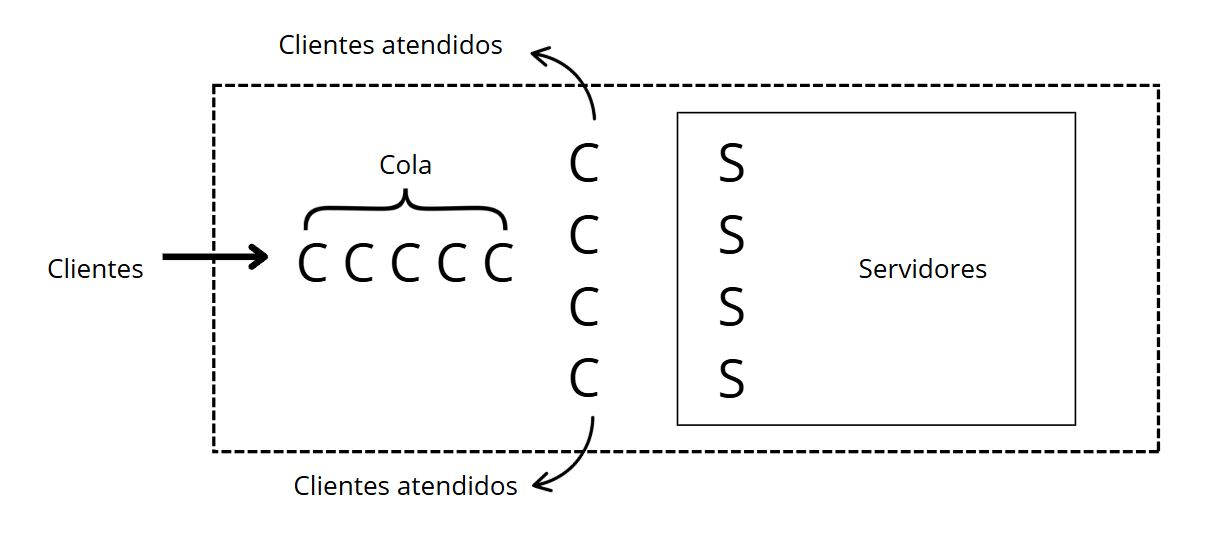
\includegraphics[width=90mm]{./images/cap1.jpg}
		\caption{Modelo.}
	\end{figure}
	\FloatBarrier

    Una vez que el paciente recibe la atención especializada, existen tres posibles desenlaces, el paciente se cura y no requiere más atención (salida del sistema), el paciente requiere seguimiento y debe regresar al hospital o el paciente abandona el tratamiento por voluntad propia. Cabe aclarar que este estudio se concentrará en el caso de la salida del sistema, puesto que asumimos un caso ideal en el que el paciente busca mejorarse y además no tiene múltiples consultas ya que eso agrandaría el flujo del sistema a estudiar.

    \section{La información y el problema general}
    Después de realizar una limpieza básica para eliminar datos innecesarios y registros vacíos, filtramos únicamente los datos correspondientes a las unidades médicas mencionadas.

    Se detectó que:
    \begin{itemize}
        \item La \textbf{UMF 66} registró \textbf{155 pacientes} el \textbf{26 de octubre de 2015}.
        \item El \textbf{Hospital 71} registró \textbf{150 pacientes} el \textbf{28 de octubre de 2015}.
    \end{itemize}

    Dado que los registros corresponden a un solo día, se asumió una jornada laboral de \textbf{12 horas} (de 8:00 a.m. a 8:00 p.m.) para calcular las tasas de llegada por hora. \\

    La tasa media de llegada (\(\lambda\)) se calcula utilizando la siguiente fórmula:

    \[
    \lambda = \frac{N}{H}
    \]

    donde:
    \begin{itemize}
        \item \(N\) = Número total de pacientes registrados.
        \item \(H\) = Número de horas de atención.
    \end{itemize}

    Aplicando la fórmula:

    \begin{itemize}
        \item \textbf{UMF 66}: \(\lambda_{UMF66} = \frac{155}{12} \approx 12.92\) pacientes por hora.
        \item \textbf{Hospital 71}: \(\lambda_{Hosp71} = \frac{150}{12} \approx 12.5\) pacientes por hora.
    \end{itemize}

    Estos valores serán utilizados para la modelación de los sistemas de colas.

\end{document}